{\color{Blue}\subsection{External Interface Requirements}}
%\subsection{External Interface Requirements}
{\color{Blue}\subsubsection{D4H: User Interfaces}}
%\subsubsection{D4H: User Interfaces}
The following figures (also the ones presented in Subsection 3.1.2 and 3.1.3) are intended to give a general idea of the final result. The final application will not be necessarily as it is presented here.
	
\begin{figure}[H]
	\centering
	\begin{minipage}[c]{.45\textwidth}
		\centering\setlength{\captionmargin}{0pt}%
		\fbox{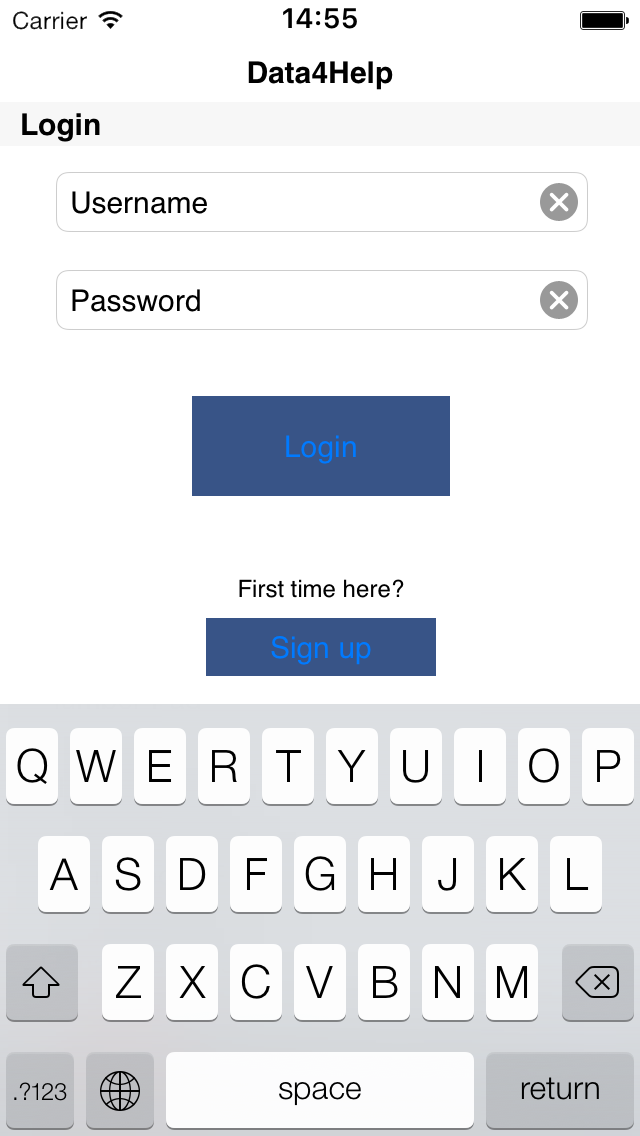
\includegraphics[scale=0.4]{Images/interfaces/Login.png}}
		\caption{User Login}
		\label{figura1}
	\end{minipage}%
	\hspace{5mm}%
	\begin{minipage}[c]{.45\textwidth}
		\centering\setlength{\captionmargin}{0pt}%
		\fbox{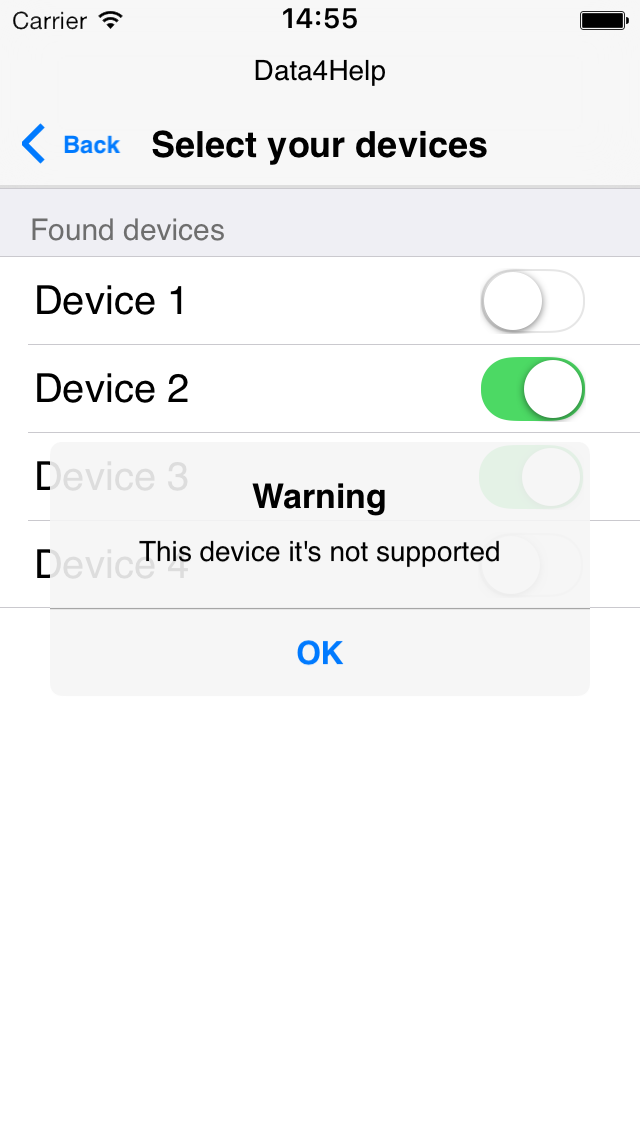
\includegraphics[scale=0.4]{Images/interfaces/SelectDevice.png}}
		\caption{Device not supported}
		\label{figura2}
	\end{minipage}
\end{figure}

\begin{figure}[H]
	\centering
	\begin{minipage}[c]{.45\textwidth}
		\centering\setlength{\captionmargin}{0pt}%
		\fbox{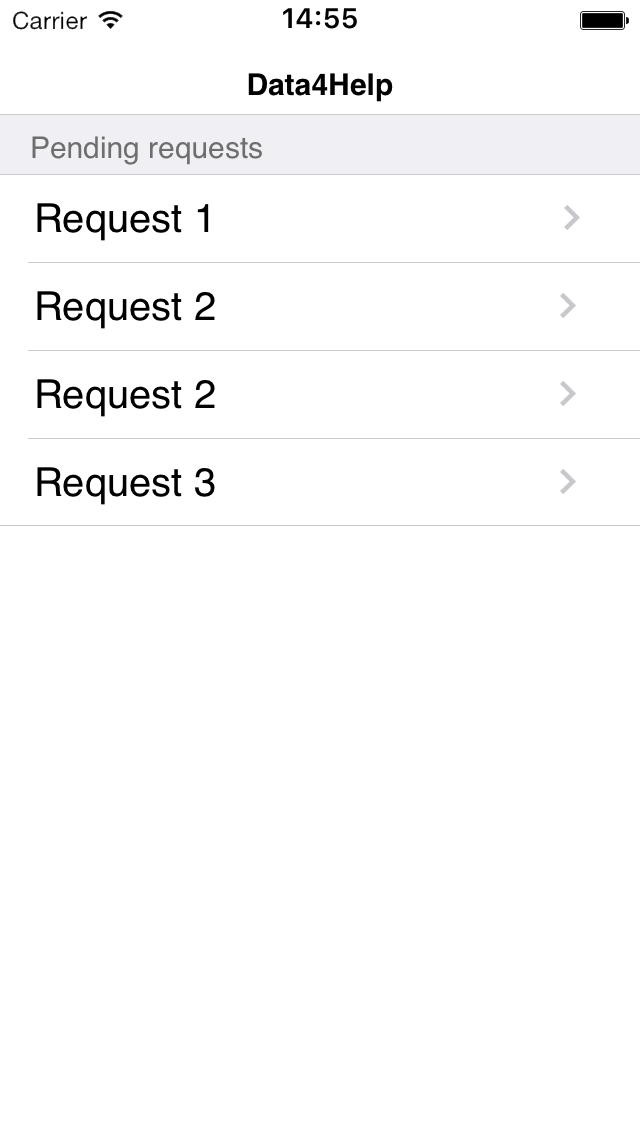
\includegraphics[scale=0.4]{Images/interfaces/PendingRequests.png}}
		\caption{Pending TP requests}
		\label{figura3}
	\end{minipage}%
	\hspace{5mm}%
	\begin{minipage}[c]{.45\textwidth}
		\centering\setlength{\captionmargin}{0pt}%
		\fbox{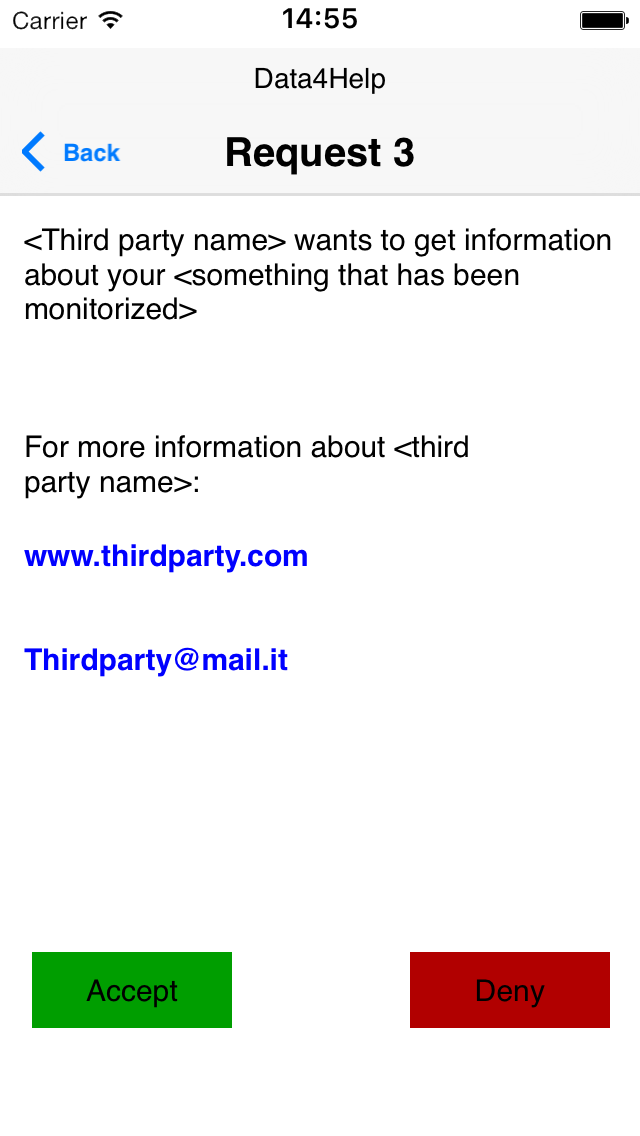
\includegraphics[scale=0.4]{Images/interfaces/TPRequest.png}}
		\caption{Evaluate Request}
		\label{figura4}
	\end{minipage}
\end{figure}

%\subsubsection{D4H: Third Party Interfaces}
{\color{Blue}\subsubsection{D4H: Third Party Interfaces}}
\begin{figure}[H]
	\centering
	\centering\setlength{\captionmargin}{0pt}%
	\fbox{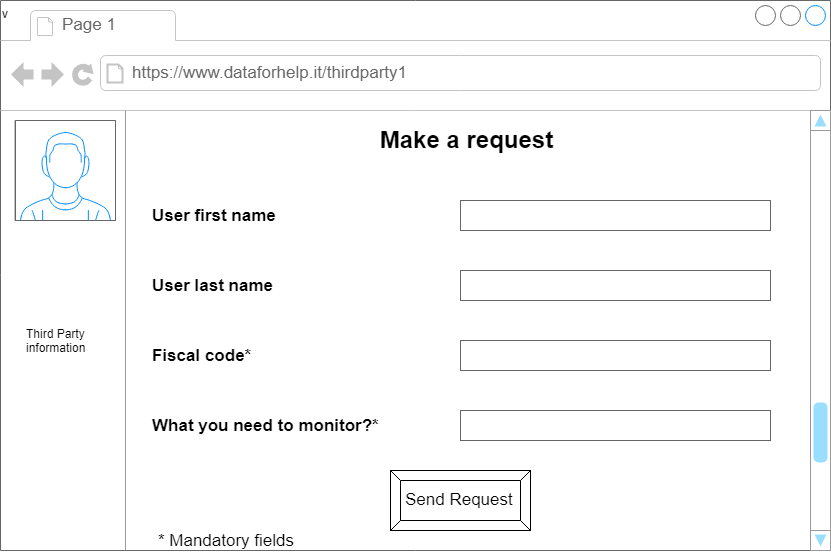
\includegraphics[scale=0.4]{Images/interfaces/MakeRequest.png}}
	\caption{TP make a request}
	\label{figura5}
\end{figure}

\begin{figure}[H]
	\centering\setlength{\captionmargin}{0pt}%
	\fbox{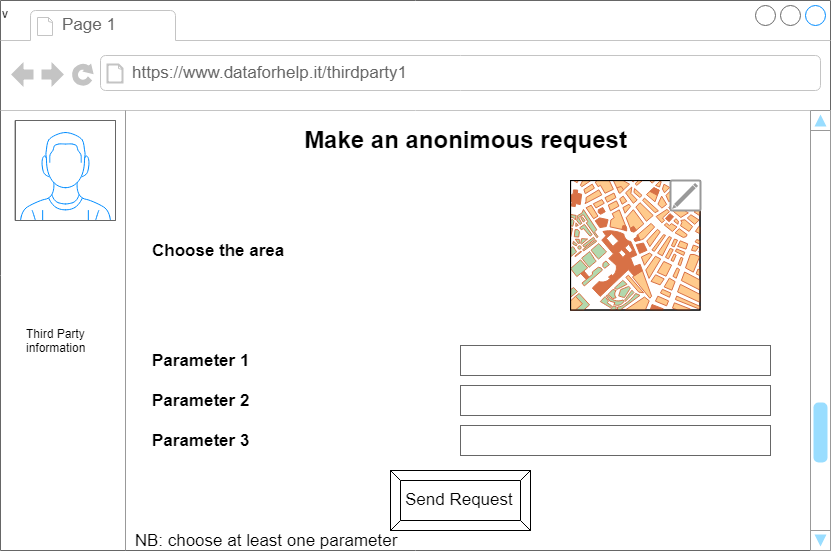
\includegraphics[scale=0.4]{Images/interfaces/AnonymousRequest.png}}
	\caption{TP make an anonymous request}
	\label{figura6}
\end{figure}

%\subsubsection{ASOS: User Interfaces}
\newpage
{\color{Blue}\subsubsection{ASOS: User Interfaces}}

\begin{figure}[H]
	\centering
	\begin{minipage}[c]{.45\textwidth}
		\centering\setlength{\captionmargin}{0pt}%
		\fbox{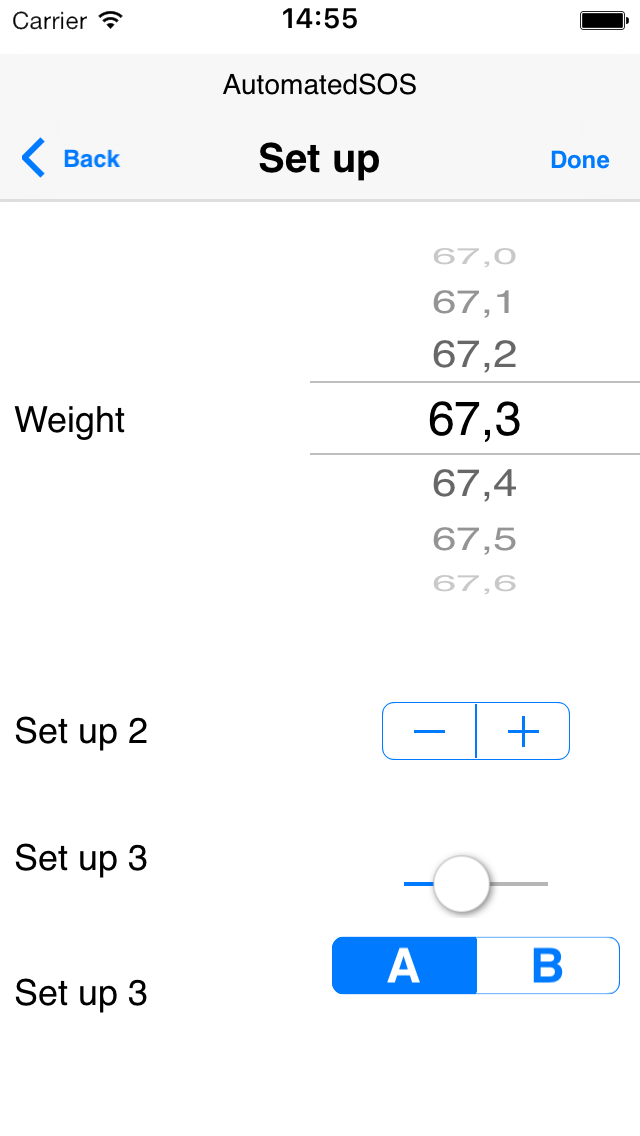
\includegraphics[scale=0.4]{Images/interfaces/Setup.png}}
		\caption{User Health Profile part 1}
		\label{figura7}
	\end{minipage}%
	\hspace{5mm}%
	\begin{minipage}[c]{.45\textwidth}
		\centering\setlength{\captionmargin}{0pt}%
		\fbox{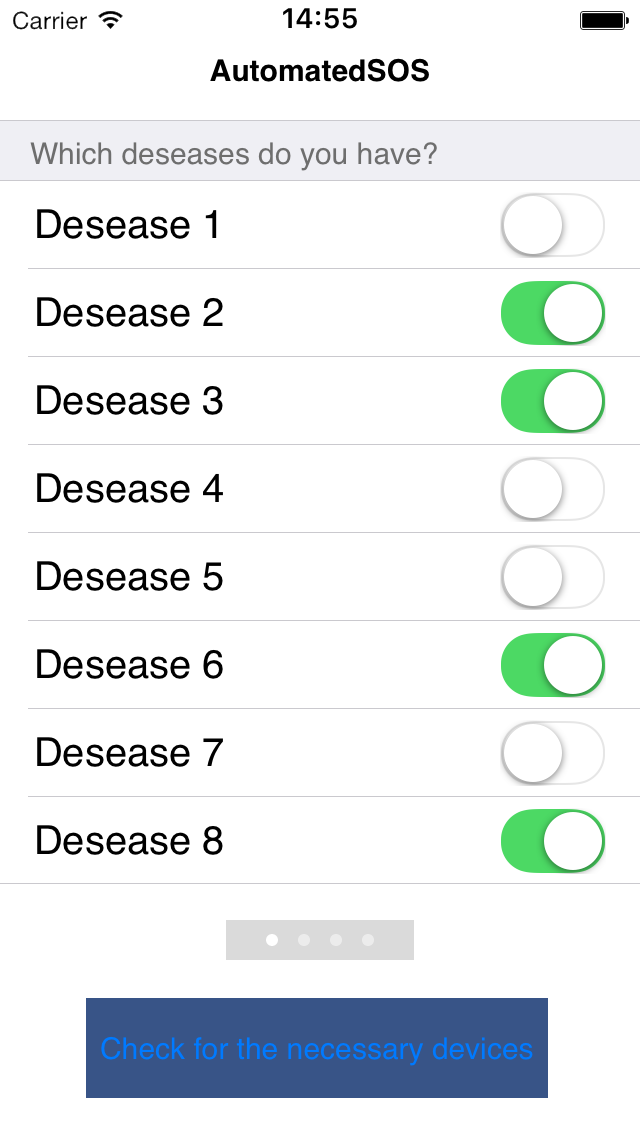
\includegraphics[scale=0.4]{Images/interfaces/SelectDesease.png}}
		\caption{User Health Profile part 2}
		\label{figura8}
	\end{minipage}
\end{figure}

\begin{figure}[htbp]
	\centering
	\begin{minipage}[c]{.45\textwidth}
		\centering\setlength{\captionmargin}{0pt}%
		\fbox{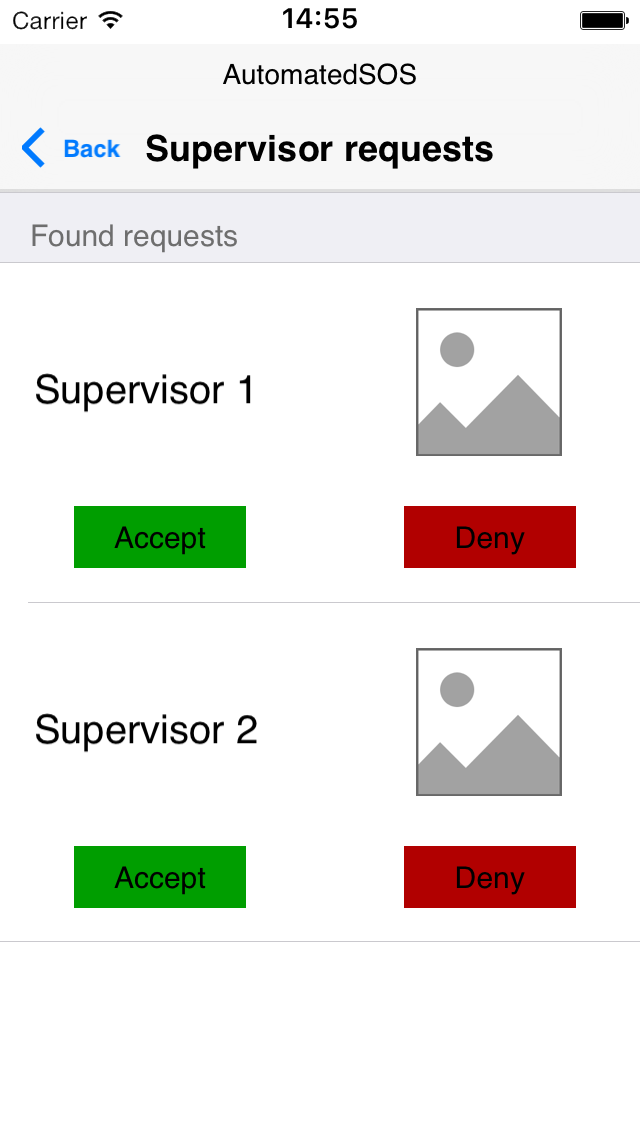
\includegraphics[scale=0.4]{Images/interfaces/Screen.png}}
		\caption{Supervisor Invitation}
		\label{figura9}
	\end{minipage}%
	\hspace{5mm}%
	\begin{minipage}[c]{.45\textwidth}
		\centering\setlength{\captionmargin}{0pt}%
		\fbox{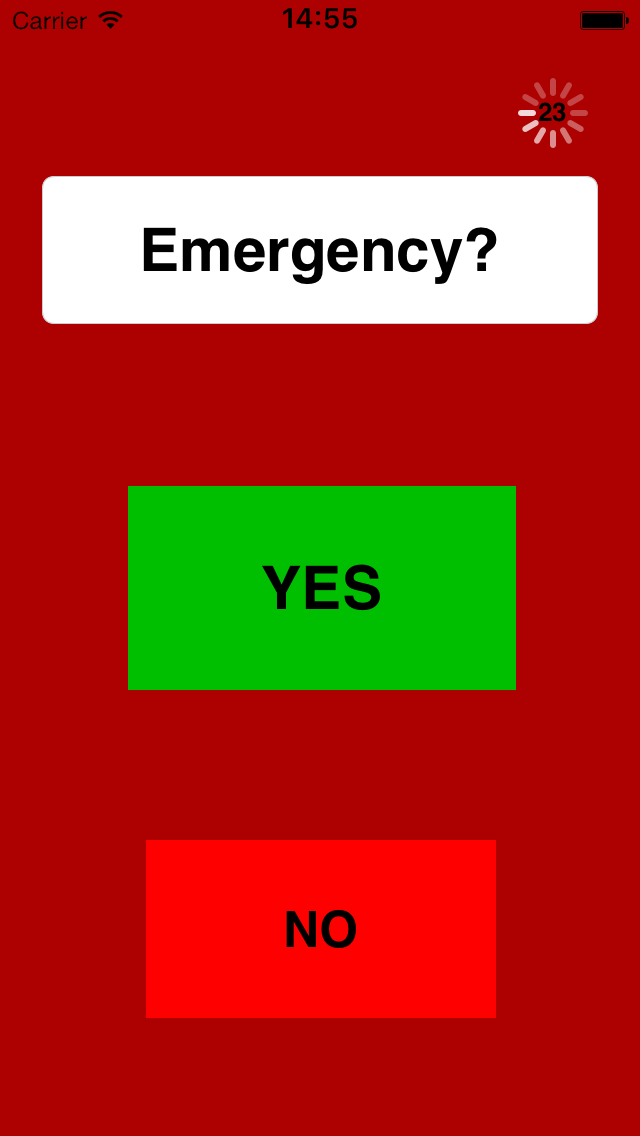
\includegraphics[scale=0.4]{Images/interfaces/EmergencyDetection.png}}
		\caption{Anomaly Detection}
		\label{figura10}
	\end{minipage}
\end{figure}
%\subsubsection{Hardware Interfaces}
{\color{Blue}\subsubsection{Hardware Interfaces}}
In order to work well and give the possibility to take advantage of the services offered by the system, both Data4Help and AutomatedSOS are required to be installed in a smartphone that provides:
\begin{itemize}
	\item GPS system
	\item Bluetooth (or BLE)
	\item NFC (Near-Field Communication)
\end{itemize} 
The first requirement is needed especially for ASOS users, as substitute of GPS bracelets or similar, in order to provide the position of the user each time the system asks for it.\\
The second requirement is important because most of the available sensor devices on the market can be connected to the smartphone using Bluetooth or BLE interfaces.\\
Sensor devices are not mandatory but strongly suggested to allow D4H to acquire health parameters (like blood pressure, HR, breath rate and so on), without them, the application does not provide consistent advantages to the users. 


%\subsubsection{Software Interfaces}
{\color{Blue}\subsubsection{Software Interfaces}}
Both the computation and the storage part of the system are completely hosted and managed by TrackMe. APIs are required to allow reading and control of the monitoring devices connected to the smartphone. This is up to the companies that decided to release open APIs or established a legal agreement with TrackMe for exploiting such interfaces.\\
Another service on which the system will rely on client side is the Bluetooth API provided by Google to simplify the management of connected sensors.\\
As mentioned in the previous sections, the system will rely on two different other external services, which as assumption will provide a proper API, they are:
\begin{itemize}
	\item \textbf{OCCA Database API:} an interface provided by the OCCA, that allows external systems to obtain information about certified organizations, from the OCCA database.
	\item \textbf{ERM System API:} it is implemented in each hospital that subscribed the ASOS project and then hosts an ERM, it allows the system to exploit the RescueSquad dispatcher that manages all the active Resources on the field 
\end{itemize}


%\subsubsection{Communication Interfaces}
{\color{Blue}\subsubsection{Communication Interfaces}}
In order to ensure confidentiality, data integrity and server authenticity, HTTP over TLS is likely to be used as network protocol to manage the encrypted communication between the client (user or third party) and TrackMe servers for security reasons. Since the protocol uses TCP at transport layer is probable to deal with problems related to delays in communication. A deep analysis of how much acceptable are such delays must be carried out.

%\subsection{Data4Help Scenarios}
{\color{Blue}\subsection{Data4Help Scenarios}}
%\subsubsection{Scenario 1}
{\color{Blue}\subsubsection{Scenario 1}}

Ross is a Dr. Herbert's patient. He discovers that the doctor is registered to Data4Help, the new service provided by TrackMe and decides to subscribe to it in order to facilitate the doctor to access his own health indicators. Ross downloads the app on his smartphone, runs it and fulfills the form for the registration. Once this procedure is completed, the service detects that a compatible smartwatch and a respiratory rate monitoring device are connected to the mobile phone through the Bluetooth interface. The application asks Ross which one he wants to register to the service. Ross selects both of them and allows the system to complete the operation.
During the evening, Dr. Herbert receives a message from Ross who confirms his registration to Data4Help. The doctor logs in the service using the hospital credentials and inserts "Ross Gilbert" in the search form. Dr. Herbert, after the system founds the user's account, formulates the request including a motivation and sends it. Ross, the morning after, runs the application and finds a notification of the awaiting request, so he checks for the requestor and accepts it.  


%\subsubsection{Scenario 2}
{\color{Blue}\subsubsection{Scenario 2}}

Angelo has bought two smart devices: an elastic strip, equipped with a sensor able to measure blood pressure, and an electronic bracelet for monitoring HR. He discovers that they can be interfaced with his smartphone through Bluetooth interface, so requests the application to register the devices. The service starts to check if the detected sensors are compatible or not. Unfortunately, only the sensor strip is completely supported by the system. So Angelo accepts to register only one device and the app, once performed the operation, update its status and return to collect data from all the connected devices.


%\subsubsection{Scenario 3}
{\color{Blue}\subsubsection{Scenario 3}}

SoftGalaxy is a software company that is working on a new application to provide to registered users a modern service called Health Advisor. It can suggest changes in daily habits, in diet and so on, according to user's data provided to the system. Unfortunately, the company cannot afford a large-scale system to collect information in real-time. In order to save as much resources as possible, it decides to rely on Data4Help to achieve this task. Before releasing the application, SoftGalaxy connects to the system and registers itself as third party, fulfilling the proper form. In addition, Data4Help asks the company to provide its digital certification for security reasons.


%\subsubsection{Scenario 4}
{\color{Blue}\subsubsection{Scenario 4}}
The company Virgin Active is considering opening a new gym near Saint Ambrogio church in Milan. In order to do so, it decides to make an anonymous request in Data4Help to receive the information about all the overweight people that live in the area of Saint Ambrogio. It receives a negative answer because there are only 593 people that suits with the requirements. Virgin Active has to change the request and so asks the same information but for a larger area, taking in also the area of Saint Agostino. This time there are enough people to let the request being forwarded and so Virgin Active can receive the information needed.


%\subsection{AutomatedSOS Scenarios}
{\color{Blue}\subsection{AutomatedSOS Scenarios}}
%\subsubsection{Scenario 1}
{\color{Blue}\subsubsection{Scenario 1}}
Michelle has an elderly mother, Teresa, who suffers about a rare heart disease. She is constantly monitored by a portable ECG device due to the high risk of being hit by a heart attack. Unfortunately, Michelle works during the morning and in this period of the day no one takes care of Teresa. She suggests to the mother to rely on AutomatedSOS, a Data4Help-based service. Since the elderly woman has a smartphone with Data4Help installed and a personal account, she decides to download the application and logs in with the Data4Help credentials. The system notices that Teresa is using the service for the first time, so it asks some information about her health problems and through it the app creates an health profile and a list of required sensors. The ECG that is actually monitoring her, is already registered and used by Data4Help, but since she has specified that suffers about loss of consciousness the system warns her that a fall sensor should be registered to provide the proper assistance. Teresa has not the device yet, so ignores the warning and complete the profiling procedure. The app finally, is ready to monitor the woman’s health status. The they after, when Michelle went to work, Teresa activated the ASOS Monitor Mode to start to be monitorated. As Michelle returned, she deactivated it.

%\subsubsection{Scenario 2}
{\color{Blue}\subsubsection{Scenario 2}}
One month ago Marianna, a 60 years old woman, decided  that  it  could  be  a  good  idea  in  order  to  live  better  and  safer to join the AutomatedSOS application.  As she was already a member of Data4Help she did not have to create a new profile but she simply logged in the new downloaded application as a Data4Help user. The system asked Marianna to  fill  a  questionnaire  about  some  basic  information  of  herself, select her diseases and register the necessary devices. Paolo, her husband, that was already an AutomatedSOS user, sends Marianna a Supervisor request that she promptly accepted. A  few  days  after,  she  had  dinner  with  friends  and  ordered  a  piece  of  cake  without  knowing  that  inside  it  there  were  almonds,  a  food  that  gives  her  anaphylactic  shock.  Immediately  she  started  to  breath  bad,  her  heartbeat  increased  and  also  her  pressure.  Her  phone  rung,  AutomatedSOS  was  asking her if  everything  was  ok.  As  Marianna  needed  an  ambulance,  she  answered  negatively.  Paolo received a notification from AutomatedSOS warning that Marianna was sick meanwhile an ambulance arrived at the restaurant, saving Marianna.   


%\subsubsection{Scenario 3}
{\color{Blue}\subsubsection{Scenario 3}}
Carol is a young student, she suffers of frequents loss of consciousness episodes due to medicines she has to take for a congenital disease. Carol is an AutomatedSOS user as well as her mother, Jenny, that decides to watch over the health conditions of her daughter when she is not home. So, Jenny in order to be notified of all the emergencies and provide support when she is not near her daughter, opens AutomatedSOS and sends to Carol an invitation for becoming her Supervisor. Carol, during the school break, receives the request and accepts it. Becoming a Supervisor, Jenny is allowed to be notified of the daughter health status when something goes wrong and to know the position of Carol.


%\subsection {Functional Requirements}
{\color{Blue}\subsection{Functional Requirements}}

%\subsubsection{Data4Help}
{\color{Blue}\subsubsection{Data4Help}}
\raggedright
\textbf{[G1]: A user can register personal health monitoring devices in the system}
\begin{itemize}[partopsep=0.7 cm]
	\item {[R1]: The system must allow a registered user to associate a sensor device to the service.}
\begin{itemize}
	\item{[D1]: The device to be registered, is supported by the system.}
\end{itemize}
\end{itemize}
\textbf{[G2]: TrackMe acquires periodically health parameters specifically related to a user}
\begin{itemize}
	\item {[R2]: Each user is uniquely identified by the system.}
	\begin{itemize}
		\item {[D2]: The user is provided with a unique identification code (such as the Fiscal Code) that allows the system to associate him/her to a real person}
	\end{itemize}
	\item {[R3]: The system can acquire health data by specific sensors connected to the user's main device.}
	\begin{itemize}
		\item {[D3]: Data acquired by the connected sensors or directly provided by the user is intended to be accurate}
		\item {[D4]: The channel for the communication between the user and the system is reliable}
	\end{itemize}
\end{itemize}

\textbf{[G3]: Third parties can access health data of specific users, if expressively authorized by them}

\begin{itemize}
	\item {[R4]: The system must be able to identify and certificate the reliability of each organization that wants to request user data.}
	\begin{itemize}
		\item {[D5]: The system has access to external resources (e.g: existing companies database) required to allow authentication and reliability evaluation of all the third parties}
	\end{itemize}
	\item {[R5]: Each registered organization that wants to access health data of specific users must be able to formulate a request providing information related to the purpose of the request.}
	\begin{itemize}
		\item {[D6]: The purpose of the request provided by the third party is intended to be truthful and accurate}
	\end{itemize} 
	\item {[R6]: The system must notify each user of a third party request as soon as it is formulated, and allow him/her to accept or reject the request.}
	\item {[R7]: For each third party request the system should provide to the user information related to the requester and the purpose of the request.}
	\item {[R8]: Once a third party request is accepted by the user, the third party must have full access to the entire collection of data of the user.}
\end{itemize}

%\raggedright
\textbf{[G4]: Third-parties can request anonymous information about groups of users}

\begin{itemize}
	\item {[R9]: Third parties must be able to request health data of groups of anonymous users, according to several criteria without being expressively authorized.}
	\item {[R10]: The system must prevent third parties to trace back to specific user information through anonymous requests.}
\end{itemize}

%\subsubsection{AutomatedSOS}
{\color{Blue}\subsubsection{AutomatedSOS}}
\raggedright
\textbf{[G5]: The user has the possibility to specify the diseases he/she has, so the system can evaluate which health parameters to monitor}

\begin{itemize}
	\item {[R11]: The system must give the possibility to the user to specify him/her health profile}
	\begin{itemize}
		\item {[D7]: The user is registered to Data4Help.}
	\end{itemize} 
	\item {[R12]: The system must prevent the possibility to use the service, if the minimum required sensors are missing.}
\end{itemize}

\textbf{[G6]: An ambulance may be sent within 5 seconds, if an emergency or anomaly condition is detected}

\begin{itemize}
	\item {[R13]: The system must allow the user to turn on and off the service each time he/she wants.}
	\item {[R14]: The system must stop monitoring when minimum required sensors are missing.}
	\item {[R15]: The system must be able to distinguish and detect emergency or anomaly conditions occurring to a specific user.}
	\item {[R16]: When an anomaly condition is detected, the system must send a notification to the user, asking if it is an emergency condition. If the user does not answer the notification within 30 seconds, the anomaly must become an emergency }
	\item {[R17]: When an emergency condition is detected, the nearest ambulance must be alerted, providing all the information about the situation.}
	\begin{itemize}
		\item {[D3]: Data acquired by the connected sensors or directly provided by the user is intended to be accurate}
		\item {[D8]: There is at least one hospital provided with an available ERM system (Emergency Resource Manager)} 
		\item {[D9]: The position of both the ambulance and the user is accurate}
	\end{itemize}
\end{itemize}
\raggedbottom
\textbf{[G7]: A user designated as Supervisor of another one, is notified of both emergency and anomaly events occurring to the supervised user}

\begin{itemize}[itemsep=0em]
	\item {[R18]: A user must have the possibility to request to become Supervisor of another one.}
	\begin{itemize}
		\item {[D10]: The Supervisor is a Data4Help registered user.}
	\end{itemize}
	\item {[R19]: Each supervised user must be able to accept or reject the possibility to have a Supervisor.}
	\item {[R20]: The Supervisor must be notified by the system of all emergency and anomaly conditions occurring to the supervised user.}
	\begin{itemize}[topsep=0em]
		\item {[D11]: The Supervisor is available when the notification is sent.}
	\end{itemize}
\end{itemize}

%\subsection{UML Modeling}
{\color{Blue}\subsection{UML Modeling}}

{\color{Blue}\subsubsection{Use Case Notation}}
In order to facilitate the comprehension of use cases, the "Exception" part of tables will contain, for each item, the corresponding step in the events flow at which the exception may be raised. Furthermore, in all the cases in which a use case is included in the description of another one, the relative part that mentions the included use case is represented underlined with a clear reference to the same one (e.g see: "Register Device"). In some tables for space and document organization needs, "Special Requirements" part has been removed, in all of these occurrences there are no special requirements. 

%\subsubsection{Data4Help Use Cases}
{\color{Blue}\subsubsection{Data4Help Use Cases}}

\begin{table}[H]
	\centering
	{\renewcommand{\arraystretch}{1.5}%
		\begin{tabular}{|@{\hspace{2em}} p{4cm} @{}| p{11cm} @{\qquad}| }
			\cline{1-2}
			\multicolumn{2}{|c|}{\textbf{User Login}} \\ \cline{1-2}
			\textbf{Actors:} & User \\ \cline{1-2}
			\textbf{Entry Conditions:} &  The user is already registered in the service \\ \cline{1-2}
			\textbf{Flow of Events:} &
			 \begin{enumerate}[itemsep=-0.2em, topsep=0em]
				\item The user inserts the access credentials
				\item The user taps on "Log in"
			\end{enumerate}\\ \cline{1-2}
			\textbf{Exit Conditions:} & The system redirect the user to his/her personal account\\ \cline{1-2}
			\textbf{Exceptions:} & 
			\begin{itemize}
				\item 2) If the credentials are not valid, the system sends a warning
			\end{itemize} \\ \cline{1-2}
	\end{tabular}} \quad
\end{table}

\begin{table}[htb]
	\centering
	{\renewcommand{\arraystretch}{2}%
		\begin{tabular}{|@{\hspace{2em}} p{4cm} @{}| p{11cm} @{\qquad}| }
			\cline{1-2}
			\multicolumn{2}{|c|}{\textbf{User Signs Up}} \\ \cline{1-2}
			\textbf{Actors:} & User \\ \cline{1-2}
			\textbf{Entry Conditions:} & The user has already downloaded the application \\ \cline{1-2}
			\textbf{Flow of Events:} & 
			\begin{enumerate}[itemsep=-0.2em, topsep=0em]
				\item The user clicks on "Signs up as User"
				\item The user inserts all the required information
				\item The user confirms the registration
				\item The system asks the user if he/she wants to 
				associate a sensor device to the service.
				\item The user accepts to register the devices
				\item The system redirect the user to the Device Registration space
				\item The user \underline{registers the devices} (see: "Register Device") connected to the smartphone
				\item The system redirect the user to his/her personal account
			\end{enumerate}\\ \cline{1-2}
			\textbf{ Conditions:} & The user is successfully signed up\\ \cline{1-2}
			\textbf{Exceptions:} & 
			\begin{itemize}[itemsep=-0.2em, topsep=0em]
				\item 3) The user is already registered to the service, a notification will be sent, preventing him/her to register again.
				\item 4) The user skips the device registration and the system redirect the user to his/her account
			\end{itemize} \\ \cline{1-2}
	\end{tabular}} \quad
\end{table}

\begin{table}[htb]
	\centering
	{\renewcommand{\arraystretch}{1.5}%
		\begin{tabular}{|@{\hspace{2em}} p{4cm} @{}| p{11cm} @{\qquad}|}
			\cline{1-2}
			\multicolumn{2}{|c|}{\textbf{Register Device}} \\ \cline{1-2}
			\textbf{Actors:} & User \\ \cline{1-2}
			\textbf{Entry Conditions:} &  The user is logged in Data4Help \\ \cline{1-2}
			\textbf{Flow of Events:} &
			 \begin{enumerate}[itemsep=-0.2em, topsep=0em]
				\item The user taps on "Add Device"
				\item The system provides the list of all the sensor devices connected to the smartphone
				\item The user selects the devices that wants to associate to the service
				\item The system registers the devices
			\end{enumerate} \\ \cline{1-2}
			\textbf{Output Conditions:} & A new monitoring device is added in the system \\ \hline
			\textbf{Exceptions:} & 
			\begin{itemize}[itemsep=-0.2em, topsep=-2em, partopsep=-1em]
				\item 4) If the registered sensor corresponds to a new monitored parameter the information is associated to the current user in the system 
				\item 4) If the device is not supported, the system sends a warning to the user and denies the device registration.
				%added 2/12/18
				\item 1) If ASOSMonitorMode is activated the system will prevent the possibility to add new devices
				\item 3) If the selected device collects the same type of data of another device already registered to the application, the user will be asked to decide which one prefers. The other one will be discarded
			\end{itemize} \\ \cline{1-2}
			\textbf{Special Requirement:} & None \\ \hline
	\end{tabular}} \quad
\end{table}

\begin{table}[H]
	\centering
	{\renewcommand{\arraystretch}{1.5}%
		\begin{tabular}{|@{\hspace{2em}} p{4cm} @{}| p{11cm} @{\qquad}|}
			\cline{1-2}
			\multicolumn{2}{|c|}{\textbf{ThirdParty Sign Up}} \\ \cline{1-2}
			\textbf{Actors:} & Third Party \\ \cline{1-2}
			\textbf{Entry Conditions:} & The third party has not registered to the service yet \\ \cline{1-2}
			\textbf{Flow of Events:} & 
			\begin{enumerate}[itemsep=-0.2em, topsep=0em]
				\item The third party clicks on "Sign Up as Third Party"
				\item The third party inserts the requested information
				\item The third party provides a certification of its identity
				\item The third party confirms the information provided
				\item The system verifies the inserted data through the OCCA open database
				\item The system confirms the registration and redirect the third party to its personal account.
			\end{enumerate}\\ \cline{1-2}
			\textbf{Exit Conditions:} & The third party is registered to Data4Help \\ \hline
			\textbf{Exceptions:} & 
			\begin{itemize}[itemsep=-0.2em, topsep=0em]
				\item 5) If the information provided is incorrect or the third party is already registered, the system shows a warning and denies the registration
			\end{itemize} \\ \hline
	\end{tabular}} \quad
\end{table}

\begin{table}[H]
	\centering
	{\renewcommand{\arraystretch}{1.5}%
		\begin{tabular}{|@{\hspace{2em}} p{4cm} @{}| p{11cm} @{\qquad}|}
			\cline{1-2}
			\multicolumn{2}{|c|}{\textbf{ThirdParty Logs in}} \\ \cline{1-2}
			\textbf{Actors:} & Third Party \\ \cline{1-2}
			\textbf{Entry Conditions:} & The third party is already registered in the service \\ \cline{1-2}
			\textbf{Flow of Events:} & \begin{enumerate}[topsep=0em, itemsep=-0.2em]
				\item The third party clicks on "Log in as Third Party"
				\item The third party inserts the access credentials
				%\item The system verifies the provided information
			\end{enumerate}\\ \cline{1-2}
			\textbf{Exit Conditions:} & The system redirects the third party to its personal account\\ \cline{1-2}
			\textbf{Exceptions:} & \begin{itemize}
				\item 2) If the inserted credentials are not valid, the system sends a warning and asks for rewrite them
			\end{itemize} \\ \cline{1-2}
			\textbf{Special Requirements:} & None \\ \cline{1-2}
	\end{tabular}} \quad
\end{table}

\begin{table}[H]
	\centering
	{\renewcommand{\arraystretch}{1.5}%
		\begin{tabular}{|@{\hspace{2em}} p{4cm} @{}| p{11cm} @{\qquad}|}
			\cline{1-2}
			\multicolumn{2}{|c|}{\textbf{Make a Request}} \\ \cline{1-2}
			\textbf{Actors:} & Third Party \\ \cline{1-2}
			\textbf{Entry Conditions:} &  The third party has already signed up for Data4Help  \\ \cline{1-2}
			\textbf{Flow of Events:} & 
			\begin{enumerate}[itemsep=-0.2em, topsep=0em]
				{\small\item The third party clicks on "Create Request"
				\item The third party selects the user data types that wants to access and inserts the information required to find the user
				\item The third party provides the motivation of the request.
				\item The system checks if someone matches the search criteria and provide the result
				\item The third party clicks on "Send Request"
				\item The system notifies the third party that the request has been sent to the user}
			\end{enumerate}\\ \cline{1-2}
			\textbf{Exit Conditions:} & The request is sent to the specific user\\ \cline{1-2}
			\textbf{Exceptions:} & 
			\begin{itemize}[topsep=-2em, itemsep=-0.2em]
				{\small\item 4) If the specified search criteria do not provide a valid result, the system shows a warning and the request is not created.}
			\end{itemize} \\ \cline{1-2}
			\textbf{Special Requirements:} & The third party knows exactly the minimum search information required to find the specific user \\ \hline
	\end{tabular}} \quad
\end{table}

\begin{table}[H]
	\centering
	{\renewcommand{\arraystretch}{1.5}%
		\begin{tabular}{|@{\hspace{2em}} p{4cm} @{}| p{11cm} @{\qquad}|}
			\cline{1-2}
			\multicolumn{2}{|c|}{\textbf{Evaluate Request}} \\ \cline{1-2}
			\textbf{Actors:} & User \\ \cline{1-2}
			\textbf{Entry Conditions:} & \begin{itemize}[itemsep=-0.2em, topsep=0em]
				\item The user is logged in Data4Help
				\item The user is notified by the system that a third party request has been received
			\end{itemize} \\ \cline{1-2}
			\textbf{Flow of Events:} & \begin{enumerate}[itemsep=-0.2em, topsep=0em]
			{\small	\item The user enters the pending requests
				\item The user selects the last request
				\item The user taps on the request 
				\item The system shows to the user identity and motivation of the requestor
				\item The user accepts the request
				\item The system notifies the third party about the decision of the user}
			\end{enumerate} \\ \cline{1-2}
			\textbf{Exit Conditions:} & The system provides the third party with the entire user's dataset\\ \cline{1-2}
			\textbf{Exceptions:} & 
			\begin{itemize}[itemsep=-0.2em, topsep=0em]
				{\small \item 3) If the request has been aborted by the third party the system notifies the user that the request is no longer acceptable or rejectable
				\item 5) If the user rejects the request, the system notifies the rejection to the third party}
			\end{itemize} \\ \cline{1-2}
			%\textbf{Special Requirements: } & None \\ \hline
	\end{tabular}} \quad
\end{table}

\begin{table}[H]
	\centering
	{\renewcommand{\arraystretch}{1.5}%
		\begin{tabular}{|@{\hspace{2em}} p{4cm} @{}| p{11cm} @{\qquad}|}
			\cline{1-2}
			\multicolumn{2}{|c|}{\textbf{Make an Anonymous Request}} \\ \cline{1-2}
			\textbf{Actors:} & Third party \\ \cline{1-2}
			\textbf{Entry Conditions:} & The third party is logged in Data4Help \\ \cline{1-2}
			\textbf{Flow of Events:} & 
			\begin{enumerate}[itemsep=-0.2em, topsep=0em]
				\item The third party clicks on "Create Anonymous Request"
				\item The third party specifies the search criteria required to find the group of anonymous users
				\item The system checks if the number of involved anonymous users are at least 1000, according the search criteria
				\item The system notifies the requestor that a valid dataset has been found
			\end{enumerate}\\ \cline{1-2}
			\textbf{Exit Conditions:} & The third party obtains the anonymous dataset \\ \cline{1-2}
			\textbf{Exceptions:} & 
			\begin{itemize} [itemsep=-0.2em, topsep=0em]
				\item 3) If the anonymous users involved in the request are less than 1000 or no one matches the search criteria, the system notifies the event and rejects the request.
			\end{itemize} \\ \cline{1-2}
			\textbf{Special Requirements:} & None \\ \hline
	\end{tabular}} \quad
\end{table}


\begin{figure}[H]
	\centering\setlength{\captionmargin}{0pt}%
	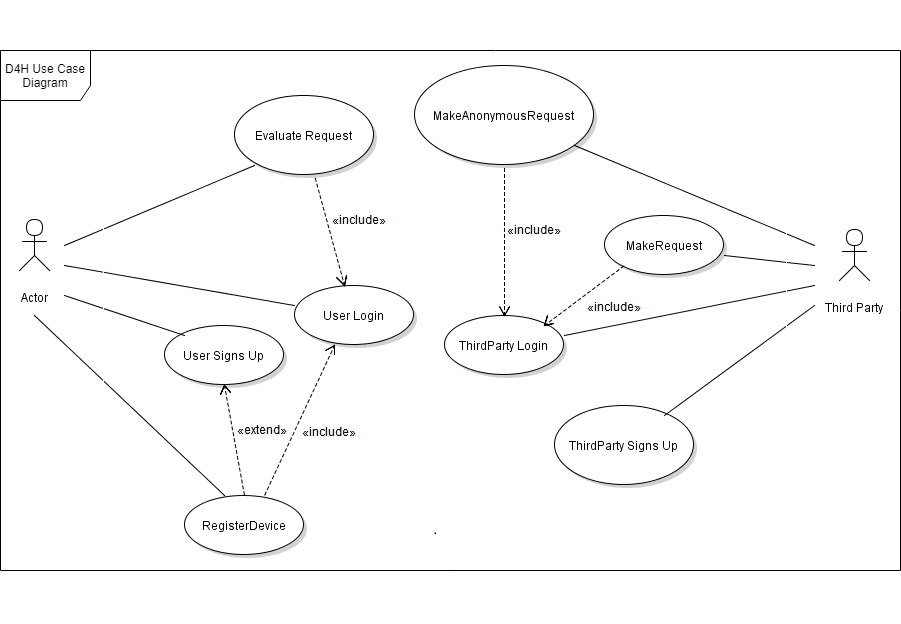
\includegraphics[scale=0.5]{Images/UML/D4H_usecase.png}
	\vspace*{-10mm}\caption{Data4Help Use Case Diagram}
	\label{figure11}
\end{figure}
\newpage
%\subsubsection{AutomatedSOS Use Cases}
{\color{Blue}\subsubsection{AutomatedSOS Use Cases}}

\begin{table}[H]
	\centering
	{\renewcommand{\arraystretch}{1.5}%
		\begin{tabular}{|@{\hspace{2em}} p{4cm} @{}| p{11cm} @{\qquad}|}
			\cline{1-2}
			\multicolumn{2}{|c|}{\textbf{User Logs in ASOS}} \\ \cline{1-2}
			\textbf{Actors:} & User \\ \cline{1-2}
			\textbf{Entry Conditions:} & The user is already registered in Data4Help \\ \cline{1-2}
			\textbf{Flow of Events:} & \begin{enumerate}[topsep=0em, itemsep=-0.2em]
				\item The user inserts the D4H access credentials
				\item The user clicks on "Log in"
				%\item The system checks if the credencials are valid
			\end{enumerate}\\ \cline{1-2}
			\textbf{Exit Conditions:} & The system redirects the user to his/her personal AutomatedSOS account\\ \cline{1-2}
			\textbf{Exceptions:} & \begin{itemize}[topsep=0em, itemsep=-0.2em]
				\item 2) If the inserted credentials are not valid, the system sends a warning and asks for rewrite them
				\item 2) If the user has logged in for the first time, the system starts to \underline{profile the health conditions of the user} (see:"Change User Health Profile")
			\end{itemize}\\ \cline{1-2}
	\end{tabular}} \quad
\end{table}

\begin{table}[H]
	\centering
	{\renewcommand{\arraystretch}{1.5}%
		\begin{tabular}{|@{\hspace{2em}} p{4cm} @{}| p{11cm} @{\qquad}|}
			\cline{1-2}
			\multicolumn{2}{|c|}{\textbf{Change Health Profile}} \\ \cline{1-2}
		   \textbf{Actors:} & User \\ \cline{1-2}
			\textbf{Entry Conditions:} & %% [topsep=0em, itemsep=-0.2em]
 The user is logged in for the first time \\ \cline{1-2}
			\textbf{Flow of Events:} & \begin{enumerate}[topsep=0em, itemsep=-0.2em]
				{\small \item  The user clicks on "Manage Health Profile"
				\item The user inserts personal information regarding age, daily habits, addictions, diagnosed diseases
				\item The system evaluates and provides a list of clinical conditions that can be monitored according to the inserted information
				\item The system checks if the sensors required for monitoring the given clinical conditions are registered to D4H and connected to the smartphone
				\item The user confirms the result }
			\end{enumerate} \\ \cline{1-2}
			\textbf{Exit Conditions:} & {\small The health profile is updated and the user is monitored according to the new clinical conditions} \\ \cline{1-2}
			\textbf{Exceptions:} & \begin{itemize}[topsep=0em, itemsep=-0.2em]
				{\small \item 3) If none of the minimum required sensors are registered or connected, the system warns the user and denies the service.
				\item 3) If only a part of the required sensors (at least the minimum required ones) are registered in the service, the user selects which of the available clinical conditions he/she wants to be monitored and confirms.
				%added 2/12/18
				\item 1) If ASOSMonitorMode is activated, the user is prevented from changing the health profile}
				\end{itemize}  \\ \cline{1-2}
	\end{tabular}} \quad
\end{table}

\begin{table}[htb]
	\centering
	{\renewcommand{\arraystretch}{1.5}%
		\begin{tabular}{|@{\hspace{2em}} p{4cm} @{}| p{11cm} @{\qquad}|}
			\cline{1-2}
			\multicolumn{2}{|c|}{\textbf{Send Supervisor Request}} \\ \cline{1-2}
			\textbf{Actors:} & User \\ \cline{1-2}
			\textbf{Entry Conditions:} & The user is logged in AutomatedSOS \\ \cline{1-2}
			\textbf{Flow of Events:} & \begin{enumerate}[topsep=0em, itemsep=-0.2em]
				\item The user clicks on "Become Supervisor"
				\item The system asks the identification of who should be supervised
				\item The user inserts the fiscal code of the supervised user
				\item The system provides the result of the research
				\item The user sends the request
			\end{enumerate}\\ \cline{1-2}
			\textbf{Exit Conditions:} & The receiver is notified of the supervisor request\\ \cline{1-2}
			\textbf{Exceptions:} & \begin{itemize}
				\item 4) If the research criteria do not match any existing AutomatedSOS user, the system sends a notification to the user
			\end{itemize} \\ \cline{1-2}
			\textbf{Special Requirements:} & None \\ \cline{1-2}
	\end{tabular}} \quad
\end{table}
\begin{table}[H]
	\centering
	{\renewcommand{\arraystretch}{1.5}%
		\begin{tabular}{|@{\hspace{2em}} p{4cm} @{}| p{11cm} @{\qquad}|}
			\cline{1-2}
			\multicolumn{2}{|c|}{\textbf{Anomaly Condition is Detected}} \\ \cline{1-2}
			\textbf{Actors:} & User\\ \cline{1-2}
			\textbf{Entry Conditions:} & \begin{itemize}[topsep=0em, itemsep=-0.2em]
				\item The user is logged in AutomateddSOS
				\item The AutomadesSOS Monitor Mode is switched on
				\item AutomatedSOS system has detected an Anomaly Condition 
				\item The ASOS Monitor Mode is activated
			\end{itemize} \\ \cline{1-2}
			\textbf{Flow of Events:} & \begin{enumerate}[topsep=0em, itemsep=-0.2em]
				\item The user is notified by the system that asks to him/her if an ambulance is needed 
				\item The user confirms that is an emergency
				\item The system turns the anomaly into an emergency condition
			\end{enumerate}\\ \cline{1-2}
			\textbf{Exit Conditions:} & The system raises an \underline{emergency condition} (see:"An Emergency Condition is Detected")\\ \cline{1-2}
			\textbf{Exceptions:} & \begin{itemize}[topsep=0em, itemsep=-0.2em]
				\item 2) If the user is fine, he/she notifies the system that an ambulance is not required
				\item 2) If the user does not reply to the notification, the anomaly timeout expires and the system alerts the nearest hospital
			\end{itemize} \\ \cline{1-2}
			\textbf{Special Requirements:} & The timeout must be fixed to 30 seconds \\ \cline{1-2}
	\end{tabular}} \quad
\end{table}

\begin{table}[H]
	\centering
	{\renewcommand{\arraystretch}{1.5}%
		\begin{tabular}{|@{\hspace{2em}} p{4cm} @{}| p{11cm} @{\qquad}|}
			\cline{1-2}
			\multicolumn{2}{|c|}{\textbf{Evaluate Supervisor Request}} \\ \cline{1-2}
			\textbf{Actors:} & User \\ \cline{1-2}
			\textbf{Entry Conditions:} &
			\setlength{\parskip}{-0.2cm}
			\setlength{\parindent}{-0.2cm} \begin{itemize}[topsep=0em, itemsep=-0.4em]
				{\small\item The user is logged in AutomatedSOS
				\item The user is notified that a Supervisor request has been received}
			\end{itemize} \\ \cline{1-2}
			\textbf{Flow of Events:} &
			\setlength{\parskip}{-0.2cm}
			\setlength{\parindent}{-0.2cm} \begin{enumerate}[topsep=0em, itemsep=-0.4em]
				{\small \item The user enters the list of the pending supervisor requests
				\item The user selects the request
				\item The system provides the identity of the requestor
				\item The user accepts the request}
			\end{enumerate}\\ \cline{1-2}
			\textbf{Exit Conditions:} & The system notifies the new Supervisor and allow him/her to access the user's health status and position during emergencies  \\ \cline{1-2}
			\textbf{Exceptions:} & 
			\setlength{\parskip}{-0.2cm}
			\setlength{\parindent}{-0.2cm}
			\begin{itemize}
				{\small\item 4) If the user rejects the request the system notifies the requestor of the refuse.}
			\end{itemize} \\ \cline{1-2}
			\textbf{Special Requirements:} & None \\ \cline{1-2}
	\end{tabular}} \quad
\end{table}



\begin{table}[H]
	\centering
	{\renewcommand{\arraystretch}{1.5}%
		\begin{tabular}{|@{\hspace{2em}} p{4cm} @{}| p{11cm} @{\qquad}|}
			\cline{1-2}
			\multicolumn{2}{|c|}{\textbf{An Emergeny Condition is Detected}} \\ \cline{1-2}
			\textbf{Actors:} & EmergencyResourceManager \\ \cline{1-2}
			\textbf{Entry Conditions:} &
			\setlength{\parskip}{-0.2cm}
			\setlength{\parindent}{-0.2cm} \begin{itemize}[topsep=0em, itemsep=-0.2em]
				{\small \item An emergency condition is detected.
				\item An anomaly is turned into an emergency condition
				\item The ASOS Monitor Mode is activated}
			\end{itemize} \\ \cline{1-2}
			\textbf{Flow of Events:} &
			\setlength{\parskip}{-0.2cm}
			\setlength{\parindent}{-0.2cm} \begin{enumerate}[topsep=0em, itemsep=-0.2em]
				{\small\item The system sends an alert to the nearest hospital's ERM providing the identification and position of the user, the reason of the emergency, the time instant at which the event has been detected
				\item The ERM alerts and dispatches that available RescueSquad which is the nearest to the user in danger}
			\end{enumerate}\\ \cline{1-2}
			\textbf{Exit Conditions:} & The system is notified that a RescueSquad has been dispatched to the user \\ \cline{1-2}
			\textbf{Exceptions:} & 
			\setlength{\parskip}{-0.2cm}
			\setlength{\parindent}{-0.2cm}
			\begin{itemize}[topsep=0cm, itemsep=-0.2em]
				{\small \item 2) If no RescueSquad for the alerted hospital is available, the system is informed about and sends the request to the ERM of the second nearest hospital, and so on if also the second attempt fails. If one of the alerted ECMs dispatches a RescueSquad for first, the system notifies the others of the dispatch.
				\item 1) If the user is associated to one or more Supervisors, these ones are also alerted of the emergency and informed of the position of the user. }
			\end{itemize} \\ \cline{1-2}
			\textbf{Special Requirements:} & The time spent between the emergency detection and the RescueSquad dispatch must be at most 5 seconds \\ \cline{1-2}
	\end{tabular}} \quad
\end{table}

\begin{table}[H]
	\centering
	{\renewcommand{\arraystretch}{1.5}%
		\begin{tabular}{|@{\hspace{2em}} p{4cm} @{}| p{11cm} @{\qquad}|}
			\cline{1-2}
			\multicolumn{2}{|c|}{\textbf{Turn on ASOS Monitor Mode}} \\ \cline{1-2}
			\textbf{Actors:} & User\\ \cline{1-2}
			\textbf{Entry Conditions:} &
			\setlength{\parskip}{-0.2cm}
			\setlength{\parindent}{-0.2cm}
			\begin{itemize}[topsep=0em, itemsep=-0.4em]
				{\small\item The user is logged in asos
					\item The ASOS Monitor Mode is off}
			\end{itemize} \\ \cline{1-2}
			\textbf{Flow of Events:} &
			\setlength{\parskip}{-0.2cm}
			\setlength{\parindent}{-0.2cm} \begin{enumerate}[topsep=0em, itemsep=-0.4em]
				{\small\item The user taps on turn on asos monitor mode
					\item The system checks if there are the minimum required sensors}
			\end{enumerate}\\ \cline{1-2}
			\textbf{Exit Conditions:} & The user starts to be monitored by the system\\ \cline{1-2}
			\textbf{Exceptions:} & 
			\setlength{\parskip}{-0.2cm}
			\setlength{\parindent}{-0.2cm}
			\begin{itemize}	
				{\small \item 2) If one or more of the minimum required sensors turn off, a notification is sent to the user and the asos monitor mode turns off}
			\end{itemize} \\ \cline{1-2}
			\textbf{Special Requirements:} & None \\ \cline{1-2}
	\end{tabular}} \quad
\end{table}

\begin{figure}[H]
	\setlength{\captionmargin}{0pt}%
	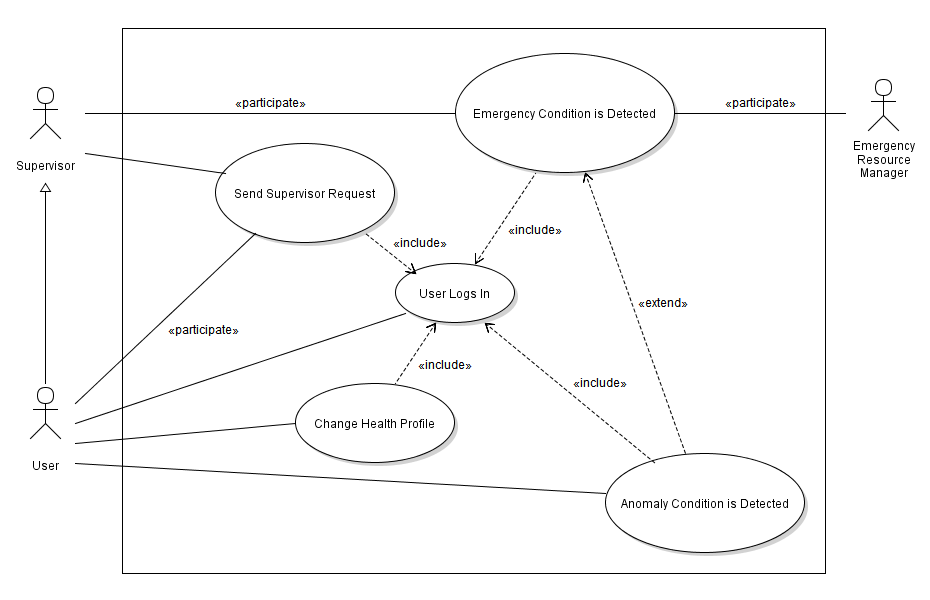
\includegraphics[scale=0.45]{Images/UML/ASOS_usecase}
	\caption{AutomatedSOS Use Case Diagram}
	\label{figure12}
\end{figure}

\newpage
%\subsubsection{Data4Help Sequence Diagrams}
{\color{Blue}\subsubsection{Data4Help Sequence Diagrams}}
\setlength{\parskip}{0.1cm}
\textbf{Register Device}
\begin{figure}[H]
	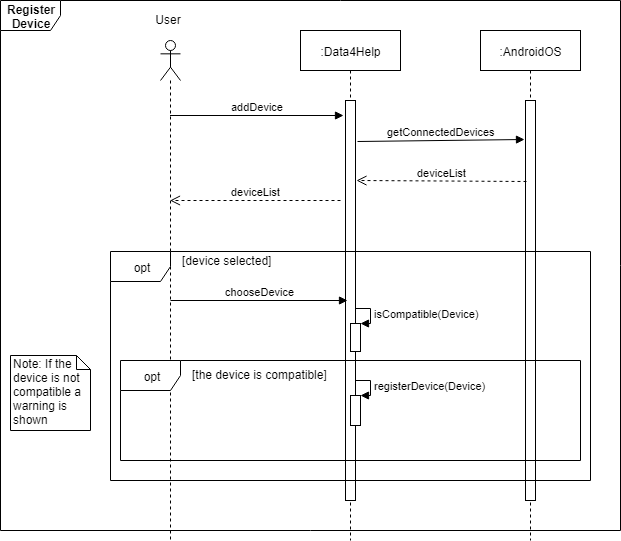
\includegraphics[scale=0.55]{Images/UML/RegisterDeviceSeq.png}
	\captionsetup{justification=raggedright, singlelinecheck=false}
	\vspace*{-2mm}\caption{Register Device Event Sequence}
	\label{figure13}
\end{figure}

\textbf{Make Request}\par
\begin{figure}[H]
	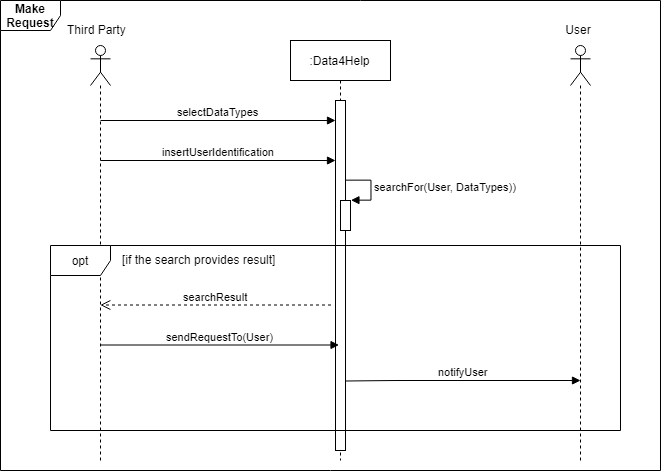
\includegraphics[scale=0.55]{Images/UML/MakeRequestSeq.png}
	\captionsetup{justification=raggedright, singlelinecheck=false}
	\vspace*{-2mm}\caption{Make Request Event Sequence}
	\label{figure14}
\end{figure}
\newpage
\textbf{Evaluate Request} \par
\begin{figure}[H]
	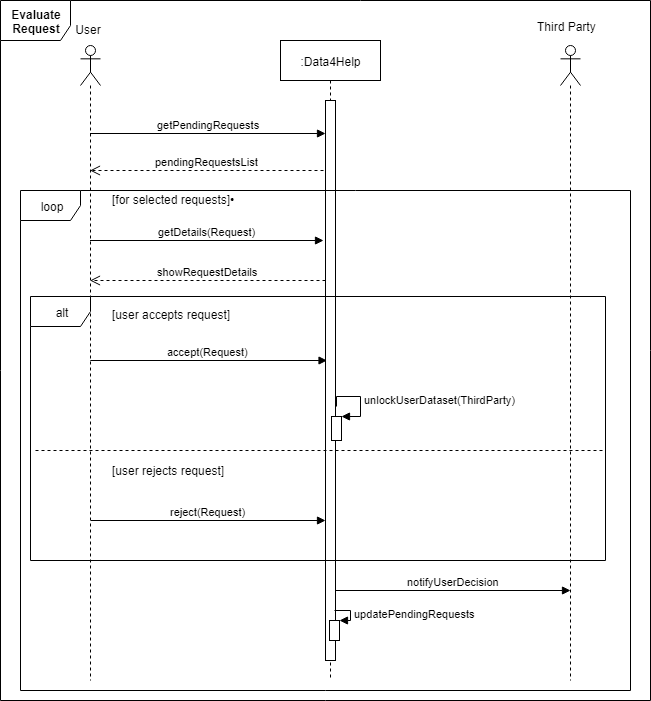
\includegraphics[scale=0.9]{Images/UML/EvaluateRequestSeq.png}
	\captionsetup{justification=raggedright, singlelinecheck=false}
	\vspace*{-2mm}\caption{Evaluate Request Event Sequence}
	\label{figure15}
\end{figure}

%\subsubsection{AutomatedSOS Sequence Diagrams}
{\color{Blue}\subsubsection{AutomatedSOS Sequence Diagrams}}

\textbf{Emergency Condition is Detected}\par
\begin{figure}[H]
	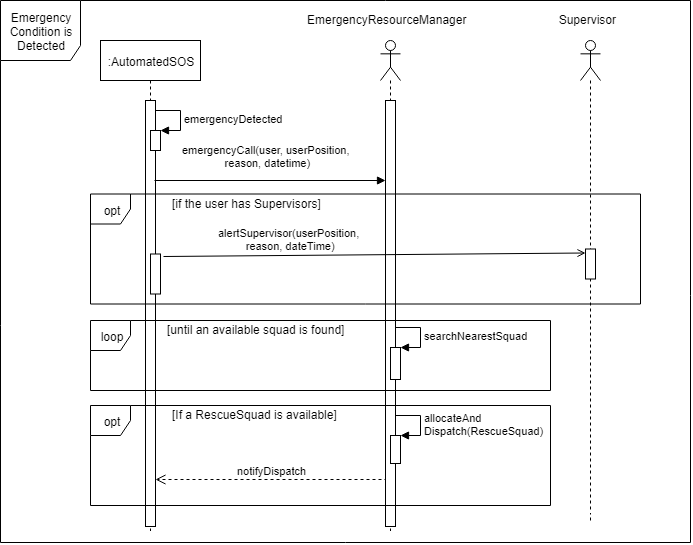
\includegraphics[scale=0.9]{Images/UML/EmergencyConditionsSeq.png}
	\captionsetup{justification=raggedright, singlelinecheck=false}
	\vspace*{-2mm}\caption{Emergency Condition Detection Event Sequence}
	\label{figure16}
\end{figure}
\newpage







\
%\subsection {Performance Requirements}
{\color{Blue}\subsection{Performance Requirements}}

Both Data4Help and AutomatedSOS aim to help the highest number of people. AutomatedSOS must guarantee that the user's information is sent in real time to the application so the emergency can be solved as soon as possible. A delay higher than 3 seconds can’t be tolerated. Data4Help have to make available the information of each user during an entire month.
\paragraph{}


%\subsection{Design Constraints}
{\color{Blue}\subsection{Design Constraints}}
Unfortunately one of the biggest limitation in the software to be is due to the large variety of monitoring devices available on the healthcare market. Companies in some cases are reluctant to provide details about the APIs of the mentioned products, since they are also involved in the development of applications able to interface with such devices in other contexts. Without a full availability of the proper libraries, it is not trivial to provide a full support to some healthcare sensors. \\
After a long evaluation, it has been decided, moreover to move the analysis of data streams related to ASOS, to the server-side application. Unfortunately, even though this solution seems to be costly in terms of computational power, it is also essential, since evaluating health conditions of an user is not a trivial task for a mobile device, it requires complex and efficient algorithms, Android OS lives in a large ecosystem of devices in certain cases so different among each other. Furthermore, this choice increases the scalability of the service, allowing the server analyzer to be enlarged in detecting dangerous health conditions for all the users. But this design decision has also a drawback, it relies entirely on the reliability of the communication channel. If some samples are lost the analysis could be affected. This side effect can be easily mitigated through a careful evaluation of the sampling frequency of the user health status in order to increase the range of visibility of critical situations.\\
There is another problem related to the connectivity. Outside the mobile and WiFi networks, it is not possible to guarantee any service. This is a critical aspect of the system. In further versions of the app, a mechanism to measure network coverage will be used to alert the user when he/she is going to be disconnected from the system when the service is turned on.\\
AutomatedSOS, in its first version, will depend strictly by the availability of the hospital ERMs. As mentioned before, this type of resource has allowed the development of AutomatedSOS. Without it, there is no possibility to alert rescue squads providing information on each raised emergency, of course the same consideration is valid for the OCCA service.

\newpage
%\subsection{Software System Attributes}
{\color{Blue}\subsection{Software System Attributes}}
%\subsubsection{Reliability}
{\color{Blue}\subsubsection{Reliability}}
Data4Help presents a critical factor related to the data processing on server side. As already motivated, this huge amount of information related to each connected user should be processed in real-time especially when supporting AutomatedSOS users, any failure of both the services could potentially lead to the death of a person. A domino effect, in which a generic fail may cause the blackout of the entire service is unacceptable and must be avoided.
\paragraph{}

%\subsubsection{Availability}
{\color{Blue}\subsubsection{Availability}}
The software has to be online 24/7, in particular the AutomatedSOS part because its chore is to guarantee a constant control of the users. In this case the system should be kept down for the least time possible when performing maintenance. For minimizing the risk of having interruption of service for patients who need assistance, an availability of at least 99.999\% has to be granted. It is an exigent but required value. Since AutomatedSOS relies on Data4Help for collecting data, both the services should have the same availability. Unfortunately this requirement is too expensive for all the users of D4H. It is sufficient to provide such level of availability only for all the users who rely on AutomatedSOS and a value of 99.99\% for the remaining ones. This solution can reduce appreciably the costs of maintenance.
\paragraph{}

%\subsubsection{Security}
{\color{Blue}\subsubsection{Security}}
Companies and organizations that want to rely on the service must certificate their identity. During the registration to D4H, they have to provide to the service a valid digital certification, released by a well-known and reliable Certification Authority. The certification after validated by the OCCA service, will be used in further communications between the TrackMe servers and Third Parties to authenticate both the parts through HTTPS protocol. This represent an essential security requirement that also provide a strong encrypted and fully authenticated communication. Since TrackMe is also provided with a digital certification, user data sent to the server will also be encrypted using TLS (Transport Layer Security). \par
Passwords of both users and third parties, must be hashed and salted on server side, a proper.
\paragraph{}

%\subsubsection{Maintainability}
{\color{Blue}\subsubsection{Maintainability}}

Especially for Data4Help, the system will deal with an enormous amount of data coming from a wide variety of sensors. Maintainability challenges will concern mainly with the support of new sensor devices appearing in the market that must be supported by the system. The architecture should facilitate the introduction of new products to speed up updated versions of the system.
\paragraph{}

%\subsubsection{Portability}
{\color{Blue}\subsubsection{Portability}}

The application has been conceived to run on Android-based devices, it will be developed in order to support all the Android smartphones with an API level higher or equal to 15 (Android 4.0, Ice Cream Sandwich).



